Here we present a brief overview of differential geometry. For a more in-depth background, we refer interested readers to \cite{do1992riemannian}, \cite{lee2003smooth}, and \cite{spivak1981comprehensive}.


%Before discussion about general regressions models for manifold-valued response variables, let's revisit manifolds.
\textbf{Differentiable manifold.}
A \textit{differentiable (smooth) manifold} of dimension $n$ is a set $\Mc$ and a maximal family of \textit{injective} mappings $\varphi_{i}:U_{i}
\subset \textbf{R}^{n} \rightarrow \Mc$ of open sets $U_{i}$ of
$\RR^{n}$ into $\Mc$ such that:
\begin{enumerate}
\item $\cup_{i}\varphi_{i}(U_{i}) =\Mc$
\item for any pair $i,j$ with $\varphi_{i} (U_{i}) \cap
\varphi_{j} (U_{j}) = W \neq \phi$, the sets $\varphi_{i}^{-1}(W)$
and $\varphi_{j}^{-1}(W)$ are open sets in $\RR^{n}$ and the
mappings $\varphi_{j}^{-1} \circ \varphi_{i}$ are
differentiable, where $\circ$ denotes function composition. 
\item The family $\{(U_{i},\varphi_{i})\}$ is maximal relative to
the conditions (1) and (2). 
\end{enumerate}

Intuitively, a differentiable (smooth) manifold $\Mc$ is a topological
space that is locally similar to Euclidean space and has a globally
defined differential structure. 

\paragraph{Tangent space ($T_{p}\Mc$).} The \textit{tangent space} at $p \in \Mc$ is a vector space which consists of 
tangent vectors of \textit{all} possible curves passing through $p$. 

\paragraph{Tangent bundle ($T\Mc$).} The \textit{tangent bundle} of $\Mc$ is the disjoint union of tangent spaces at all points of $\Mc$, 
$T\Mc = \coprod_{p \in \Mc}T_{p}\Mc$. 
The tangent bundle is equipped with a natural \textit{projection map} $\pi: T\Mc \rightarrow \Mc$. 

\paragraph{Riemannian manifold.} A \textit{Riemannian manifold} is 
%a differentiable manifold which is 
equipped with a
smoothly varying metric (inner product), the \textit{Riemannian metric}. 

Various classical geometric notions, e.g., the angle between two curves 
or the length of a curve, can be extended to manifold spaces.

\paragraph{Geodesic curves.} A geodesic curve on a Riemannian manifold is the locally shortest (distance-minimizing) curve.
These are analogous to straight lines in Euclidean space 
and a main object to generalize linear models to Riemannian manifolds (as we will in Chapter~\ref{chap:covtraj}).

\paragraph{Geodesic distance.} The \textit{geodesic distance}
between two points on $\Mc$ is the length of the shortest {\em geodesic} curve connecting the two points. More generally, distance between two points on Riemannian manifolds is defined by the infimum of the length of all differentiable curves connecting the two points. Let $\gamma$ be a continuously differentiable curve $\gamma:[a,b] \rightarrow \Mc$ between $p$ and $q$ in $\Mc$ and $g$ be a metric tensor in $\Mc$.
Then, formally, the distance between $p$ and $q$ is defined as
\begin{equation}
\text{d}(p,q) := \inf_\gamma \int_a^b \sqrt{g_\gamma(t) (\dot{\gamma}(t), \dot{\gamma}(t))} dt
\end{equation}
where $\gamma(a)=p$ and $\gamma(b)=q$, and $\dot{\gamma}$ is the derivative or rate of change of $\gamma$.
%Such shortest curves are
%known as \textit{geodesic} and are analogous to straight lines in
%. 

\paragraph{Exponential map}. An exponential map is a map from a tangent space $T_p\Mc$  to $\Mc$, which is usually locally defined due to the existence and uniqueness of an ordinary differential equation for the map.
The geodesic curve from $y_i$ to $y_j$ can be parameterized by a tangent vector in the tangent space at $y_i$ with an exponential map $\EXP(y_i,\cdot ): T_{y_i}\Mc \rightarrow \Mc$. 

\paragraph{Logarithm map.}
The inverse of the exponential map is the \textit{logarithm map}, $\LOG(y_i,\cdot):\Mc \rightarrow T_{y_i}\Mc$. 
For completeness, Table \ref{tab:comp} shows corresponding operations in the Euclidean space and Riemannian manifolds.
In what follows, when operations are nested, the exponential map and its inverse logarithm map are denoted by $\EXP(p, x)$ and $\LOG(p, v)$ respectively, where $p, x \in \Mc$ and $v\in T_p\Mc$. They are usually denoted $\EXP_p(x)$ and $\LOG_p(v)$ in classical differential geometry literature. 
 
Separate from the above notations, the matrix exponential, i.e, $\exp(X):= \sum \frac{1}{k!} X^k$, where $0!=1$ and $X^0=I$  and the matrix logarithm are denoted fully lowercase by as $\exp(\cdot)$ and $\log(\cdot)$, similar to their univariate counterparts. These will be necessary in a specific instance in Chapter~\ref{chap:covtraj}, but otherwise will refer
to the common univariate functions in other contexts.
\todo{projection in figure should be curved probably, shift the tangent a bit right/down}
\begin{figure}
	\centering
	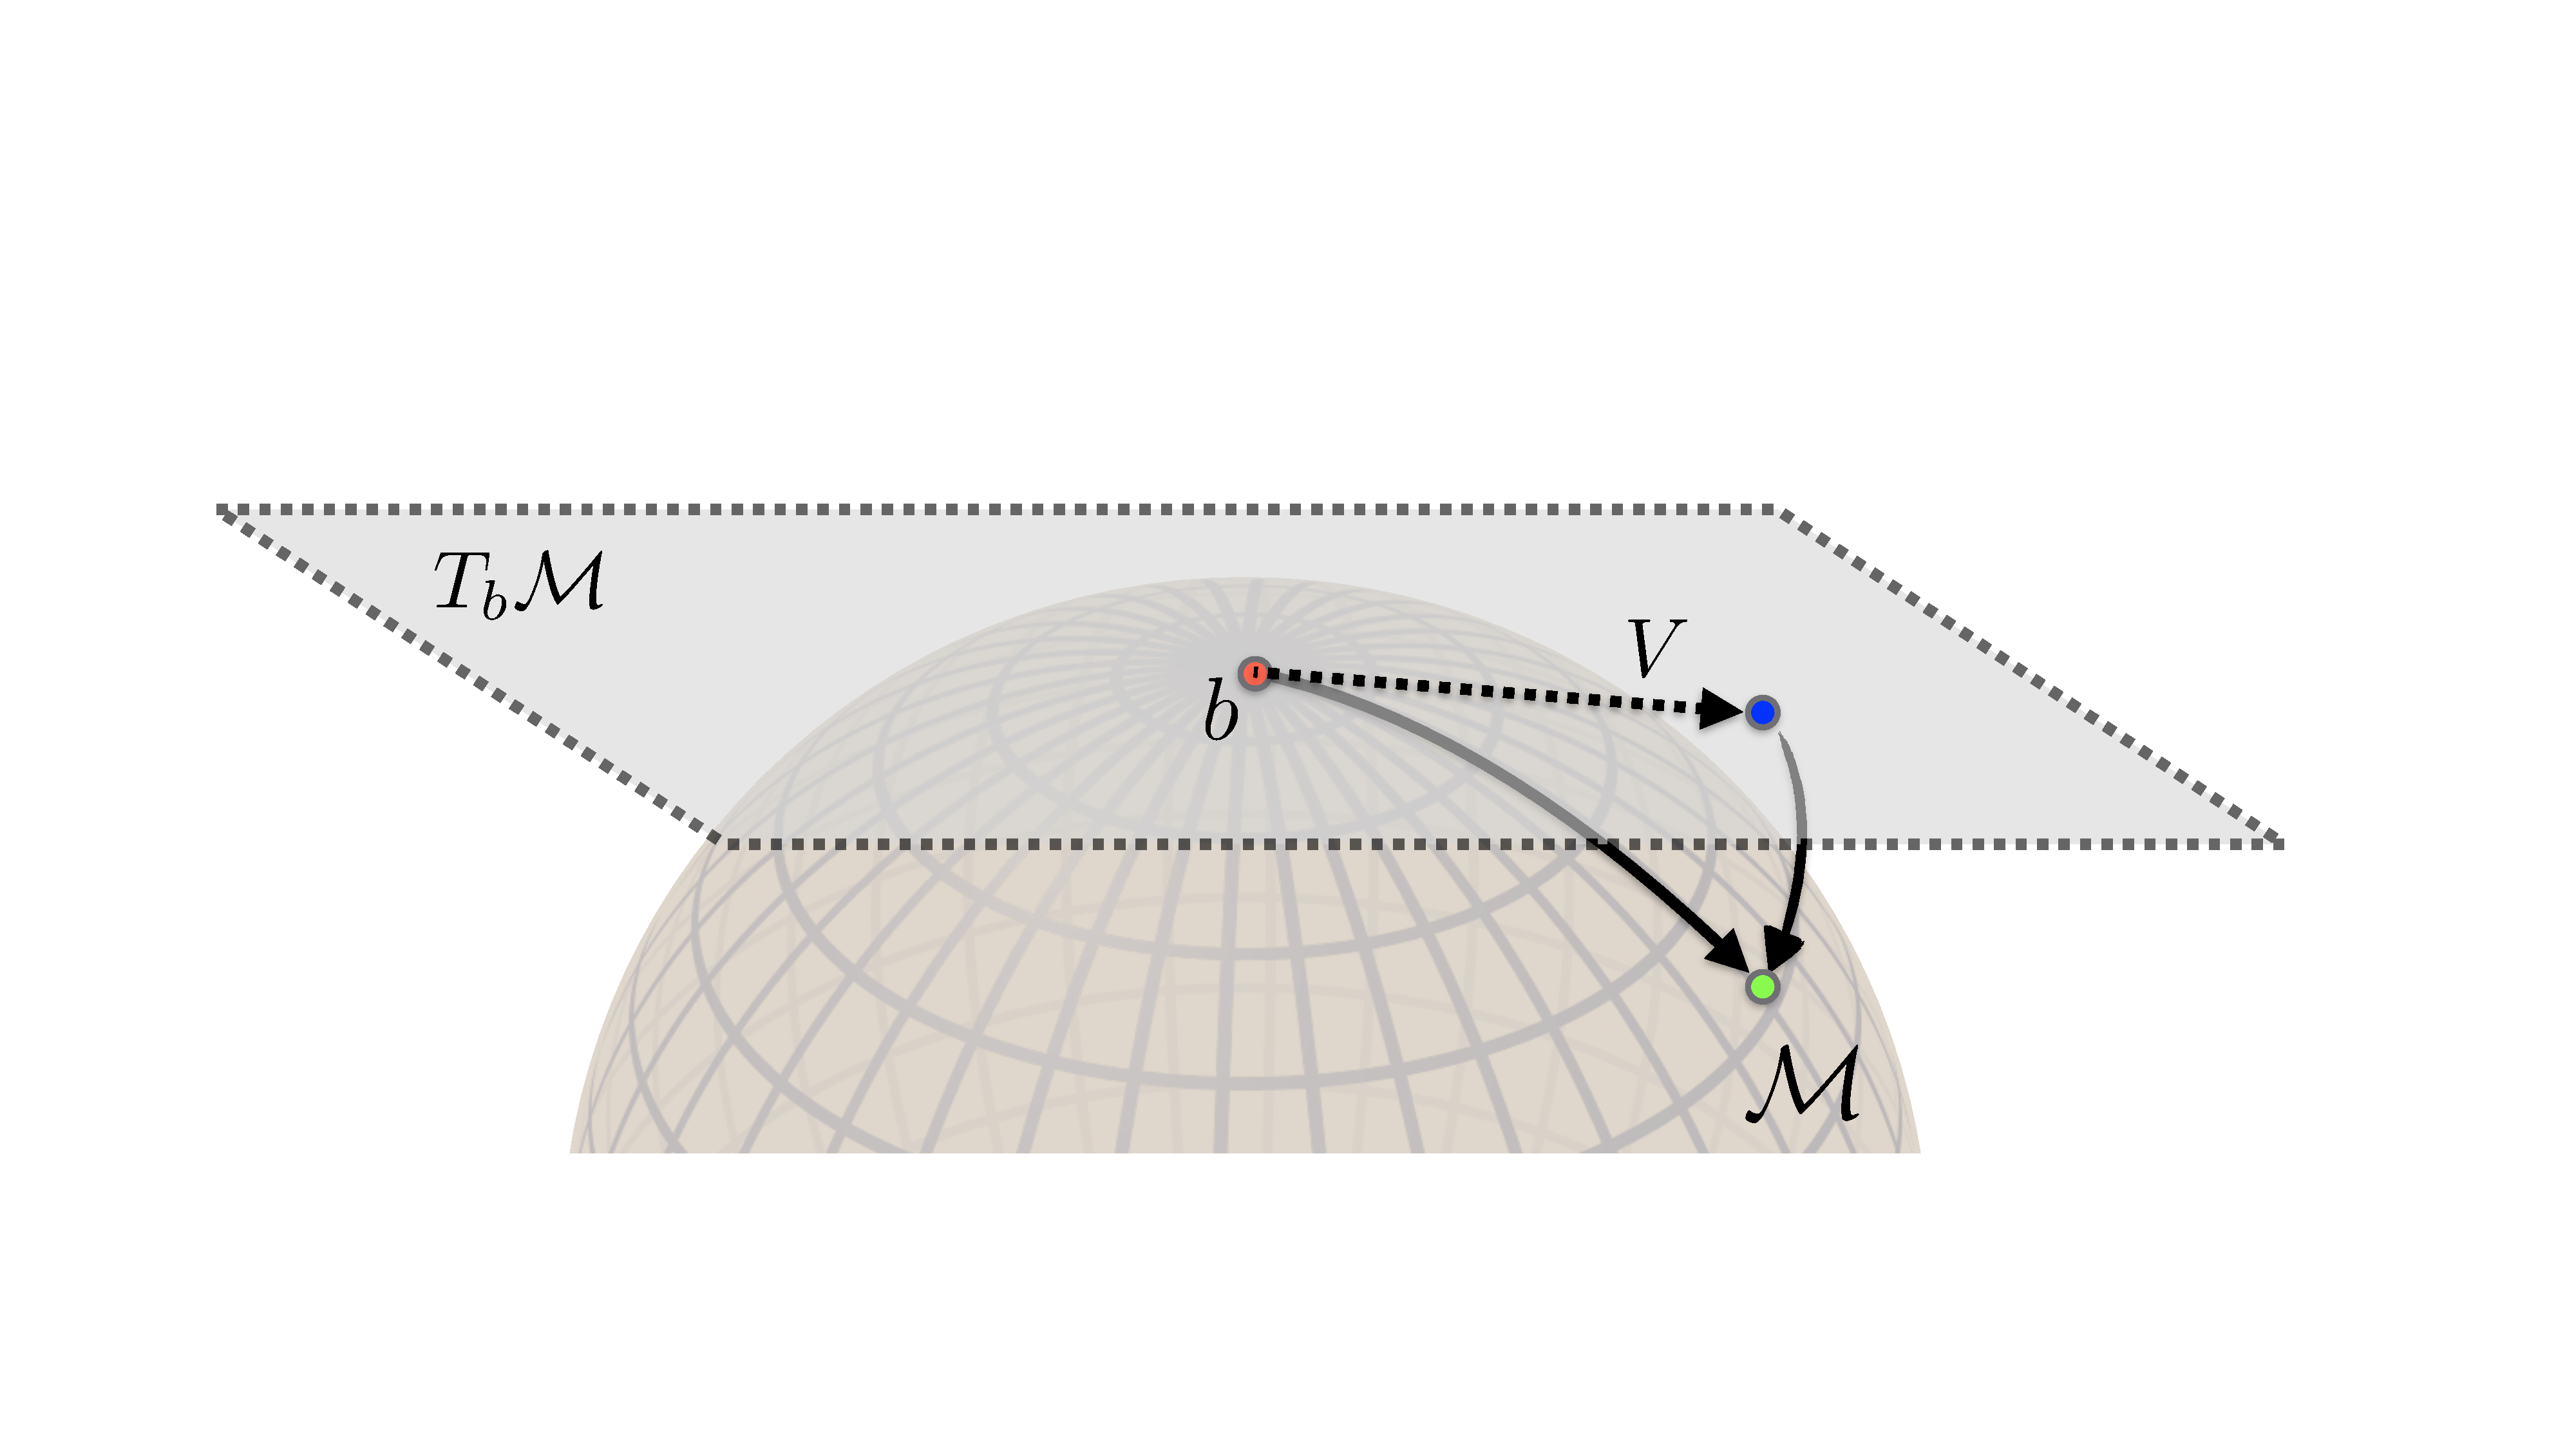
\includegraphics[width=\textwidth,trim={0 7cm 5cm 10cm},clip]{2_bknd/manifoldops.pdf}
	\caption[Operations on the Manifold]{From a basepoint $b$, we can identify the tangent space $T_b\cM$, use a direction $V\in T_b\cM$ to move using the tangent map, and use the exponential map to project back on to the manifold.}
	\label{fig:ot}
\end{figure}

% \renewcommand{\arraystretch}{1.5}
% \begin{table}
% {\footnotesize
% \begin{center}
%     \begin{tabular}{| l | l | l | }
%     \hline
%     Operation & Euclidean & Riemannian  \\  \hline 
%     \footnotesize Subtraction $\overrightarrow{x_i x_j}$& $x_j - x_i$ & $\LOG(x_i,x_j)$ \\ 
%     \footnotesize Addition $x_i+\overrightarrow{x_j x_k}$& $x_i + \overrightarrow{x_j x_k}$ & $\EXP(x_i,\overrightarrow{x_j x_k})$ \\     
%     \footnotesize Distance$(x_{i},x_{j})$  & $\| \overrightarrow{x_i x_j} \|$ & $\|\LOG(x_i,x_j) \|_{x_i}$ \\ 
%     Mean $\bar{x}$ & $\sum_{i=1}^{n} \overrightarrow{\bar{x}x_{i}}=0$ & \footnotesize $\sum_{i=1}^{n} \LOG(\bar{x}, x_i)=0$  \\ 
%     Covariance$(x)$ & \footnotesize$\E \left [ (x_i - \bar{x})(x_i - \bar{x})^{T} \right ]$&\footnotesize $\E \left [ \LOG(\bar{x}, x)\LOG(\bar{x}, x)^{T} \right ]$\\ [1ex] \hline 
%   \end{tabular}
% \end{center}
% }
% \caption{Basic operations in Euclidean space and Riemannian manifolds.}
% \label{tab:comp}
% \end{table}
\begin{table}
\begin{center}
    \begin{tabular}{| l | l | l | }
    \hline
    Operation & Euclidean & Riemannian  \\  \hline 
    \footnotesize Subtraction & $\overrightarrow{x_i x_j} = x_j - x_i$ & $\overrightarrow{x_i x_j} = \LOG(x_i,x_j)$ \\ 
    \footnotesize Addition & $x_i + \overrightarrow{x_j x_k}$ & $\EXP(x_i,\overrightarrow{x_j x_k})$ \\     
    \footnotesize Distance  & $\| \overrightarrow{x_i x_j} \|$ & $\|\LOG(x_i,x_j) \|_{x_i}$ \\ 
    Mean  & $\sum_{i=1}^{n} \overrightarrow{\bar{x}x_{i}}=0$ & \footnotesize $\sum_{i=1}^{n} \LOG(\bar{x}, x_i)=0$  \\ 
    Covariance & \footnotesize$\EE \left [ (x_i - \bar{x})(x_i - \bar{x})^{T} \right ]$&\footnotesize $\EE \left [ \LOG(\bar{x}, x)\LOG(\bar{x}, x)^{T} \right ]$\\ [1ex] \hline 
  \end{tabular}
\end{center}
\caption[Basic operations on Riemannian manifolds]{Basic operations in Euclidean space and Riemannian manifolds.}
\label{tab:comp}
\end{table}
\todo{match table formatting elsewhere, maybe}

\paragraph{Intrinsic mean.} 
Let $d(\cdot,\cdot)$ define the distance between two points. The intrinsic (or Karcher) mean is the minimizer to
\begin{equation}\label{eq:karchermean}
\bar{y} = \arg \min_{y \in \Mc} \sum_{i=1}^{N} d(y,y_{i})^{2}, 
\end{equation}
which may be an arithmetic, geometric or harmonic mean depending on $d(\cdot,\cdot)$.
A Karcher mean is a local minimum to \eqref{eq:karchermean},
and a global minimum is referred to as a Fr\'{e}chet mean.
On manifolds, the Karcher mean satisfies $\sum_{i=1}^{N} \LOG_{\bar{y}}y_i =0$.
\begin{algorithm}
	\caption{Karcher Mean on Manifolds}\label{alg:karcher}
	\SetAlgoLined
	\DontPrintSemicolon
	\KwIn{$y_{1}, \ldots, y_{N} \in \Mc$, $\alpha$}
	\KwOut{$\bar{y} \in \Mc$}
	\While{$ \| \sum_{i=1}^{N} \LOG(\bar{y}_{k},y_{i})\| > \epsilon$}{
		$\Delta\bar{y} = \frac{\alpha}{N} \sum_{i=1}^{N}\LOG (\bar{y}_k,y_i)$;\\
		$\bar{y}_{k+1} = \EXP(\bar{y}_k,\Delta \bar{y})$
	}
\end{algorithm}
This identity implies the first order necessary condition of \eqref{eq:karchermean},
i.e., $\bar{y}$ is a local minimum with a zero norm gradient \citep{karcher1977riemannian}.
In general, on manifolds, the existence and uniqueness of the Karcher mean is not guaranteed
unless we assume, for uniqueness, that the data is in a small neighborhood.

\paragraph{Parallel transport.} 
Let $\Mc$ be a differentiable manifold with an affine connection $\nabla$ and $I$ be an open interval.
Let $c:I \rightarrow \Mc$ be a differentiable curve in $\Mc$
and let $V_0$ be a tangent vector in $T_{c(t_0)}\Mc$, where $t_{0} \in I$. 
Then, there exists a unique parallel vector field $V$ along $c$, such that $V(t_0)=V_0$.
Here, $V(t)$ is called the \textit{parallel transport} of $V(t_0)$ along $c$. 

\subsection{Geometry of SPD manifolds}
As mentioned above, covariance matrices are symmetric positive definite matrices.
Here we focus our discussion to the above operations specific to SPD matrices.
 
Let SPD($n$) be a manifold for symmetric positive definite matrices of size $n\times n$.
This forms a quotient space $GL(n)/O(n)$, where
$GL(n)$ denotes the general linear group (the group of $(n \times n)$ nonsingular matrices)
and $O(n)$ is the orthogonal group 
(the group of $(n \times n)$ orthogonal matrices). 
Here, the tangent space $T_{p}\Mc$ is the space of symmetric matrices of dimension $(n+1)n/2$.

The inner product of two tangent vectors $u,v \in T_{p}\Mc$ is given by 
\begin{equation}
\begin{split}
  \langle u,v \rangle_{p} = \tr(p^{-1/2}up^{-1}vp^{-1/2})
\end{split}
\label{eq:metricSPD}
\end{equation}
This plays the role of the Fisher-Rao metric in the statistical model of multivariate distributions.
The geodesic distance is $d(p,q)^{2} = \tr( \log^{2}(p^{-1/2}qp^{-1/2}))$.

The exponential maps and logarithm maps are given as 
\begin{equation}
\begin{split}
  \EXP(p,v) = p^{1/2} \exp(p^{-1/2}vp^{-1/2})p^{1/2}, \;\;
  \LOG(p,q) = p^{1/2} \log(p^{-1/2}qp^{-1/2})p^{1/2}.
\end{split}
\end{equation}
Let $p, q$ be in SPD($n$) and a tangent vector $w \in T_{p}\Mc$, the
tangent vector in $T_{q}\Mc$ which is the parallel transport of $w$ along
the shortest geodesic from $p$ to $q$ is given by 
\begin{equation}
\begin{split}
\Gamma_{p \rightarrow q}(w) &= p^{1/2}rp^{-1/2}wp^{-1/2}rp^{1/2} \\
\text{where } r &= \exp \left (p^{-1/2}\frac{v}{2}p^{-1/2} \right ) \text{ and
}v = \LOG(p,q)
\end{split}
\end{equation}

\paragraph{Other spaces of interest.}
Orthogonal matrices of fixed size and rank also form a manifold, the (compact) \textbf{Stiefel Manifold}: $ \ST(p,n)=\left\{Y \in \RR^{n\times p} | Y^TY=I_p,\: p \leq n\right\}$.
An arbitrary $X \in \RR^{n \times p}$ matrix can be projected onto the Stiefel manifold $\ST(p,n)$ using $X \mapsto UV^T$ where $X=U\Sigma V^T$ is the (thin) singular value decomposition of $X$. We will use this fact in Chapter~\ref{chap:ott}.